\section{Experimental Results}

For our experiments, we have implemented \textsf{PCStream} in the Linux kernel
4.5.  For objective evaluation, we compared \textsf{PCStream} with three
existing schemes: \textsf{Baseline}, \textsf{Manual}~\cite{MultiStream}, and
\textsf{AutoStream}~\cite{AutoStream}.  \textsf{Baseline} stands for a legacy
SSD that does not support a multi-stream feature. \textsf{Manual} is a RocksDB
implementation which is manually optimized for multi-streamed SSDs.
\textsf{AutoStream} is an LBA-based data separation technique which is
implemented at the block driver layer. To understand the impact of the
two-phase assignment, in addition, we compared \textsf{PCStream} with
\textsf{PCStream$^{*}$} which excluded the two-phase assignment feature.

For benchmarks, we have used three scenarios of \texttt{db\_bench} of RocksDB:
Update-Random (\texttt{UR}), Append-Random (\texttt{AR}), and Fill-Random
(\texttt{FR}) scenarios.  For key-value pairs already stored in the SSD,
\texttt{UR} updates values for random keys, creating many
read-modify-writes in the SSD.  \texttt{AR} is similar to \texttt{UR}, except
that it performs the update of values for growing keys. \texttt{FR} writes
key-value pairs to the SSD in a random key order.

\subsection{Experiments with the emulator}

\begin{figure}[t]
	\centering
	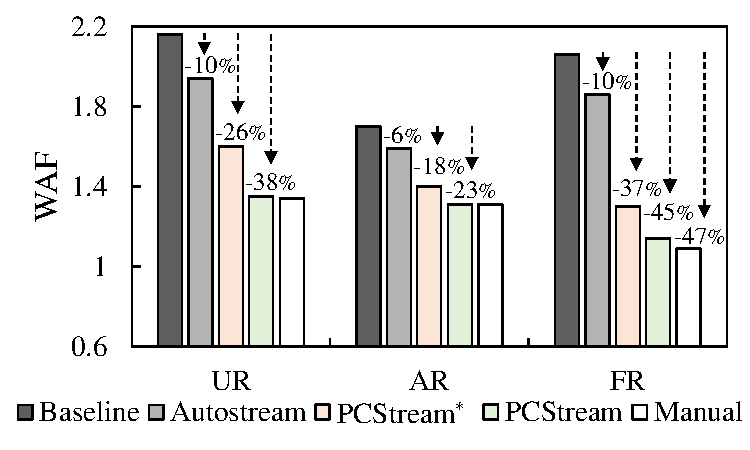
\includegraphics[width=1\linewidth]{figure/result_emul}
	\vspace{-10pt}
	\caption{The WAF comparison on the emulator.}
	\label{fig:result_emul}
	\vspace{-15pt}
\end{figure}

We carried out a set of experiments using an SSD emulator which is based on the
open flash development platform~\cite{AMF}.  The SSD emulator emulates the
behaviors of an SSD using host DRAM in the kernel level. Thus, it not only
allows us to easily add new features, but enables to analyze detailed internal
activities of an SSD.  We enhanced the original emulator so that it supported a
multi-streamed feature as well as the two-phase stream assignment.  The number
of streams supported by the emulator was 8.  The SSD emulator provided 12 GB
capacity with 4 channels and 4 ways, and there were 8192 flash blocks, each of
which was composed of 384 4-KB pages.  

We compared WAF of the existing techniques with {\sf PCStream} for the three
scenarios, and the result is shown in Fig.~\ref{fig:result_emul}.  As shown in
Fig.~\ref{fig:result_emul}, {\sf PCStream$^*$} reduced WAF by up to 30\% over
\textsf{AutoStream}.  The result shows that separating short-lived data (e.g.,
log and flush) from long-lived one (e.g., compaction) using PC was quite
effective in reducing WAF.  Moreover, {\sf PCStream} showed similar WAF to
\textsf{Manual}, reducing it by up to 38\% over \textsf{AutoStream}.  This
additional benefit came from isolating long- and short-lived data in separate
blocks through the two-phase assignment at the SSD even if they belonged to the
same compaction PC.

\textcolor{red}{(TODO: please add text for new exp here)}

\subsection{Experiments with the SSD}
\begin{figure}[t]
	\centering
	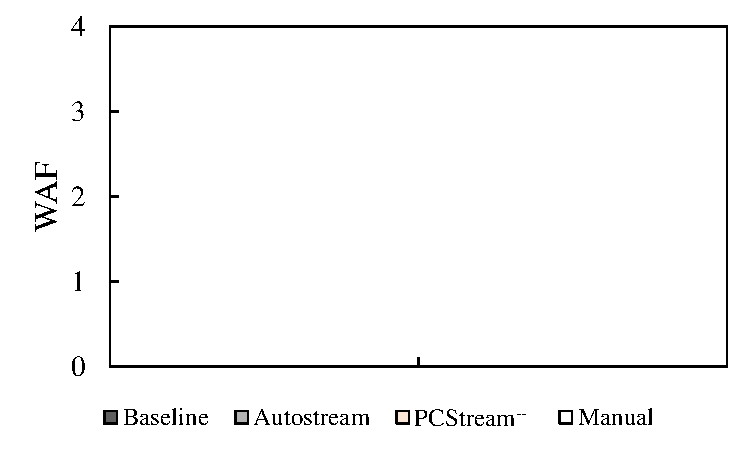
\includegraphics[width=1\linewidth]{figure/result_ssd}
	\vspace{-10pt}
	\caption{The WAF comparison on the SSD.}
	\label{fig:result_SSD}
	\vspace{-15pt}
\end{figure}

In order to confirm the feasibility of \textsf{PCStream}, we also have
conducted experiments using Samsung's PM963 480GB SSD that supports 8 streams.
Since it was impossible to implement the two-phase stream assignment in the
commercial SSD firmware, we evaluated {\sf PCStream$^*$} only.  To warm up the
SSD before running benchmarks, we filled up 90\% of the SSD capacity with valid
data.

As illustrated in Fig.~\ref{fig:result_SSD}, {\sf PCStream$^*$} reduced WAF by
30\% over \textsf{AutoStream} on average. Even though \textsf{AutoStream} on
the SSD performed better than on the emulator, {\sf PCStream$^*$} still
outperformed \textsf{AutoStream}, confirming the feasibility of the PC-based
data separation on real-world SSDs.  We also expect that {\sf PCStream} would
be able to achieve WAF closer to \textsf{Manual} once the two-phase assignment
is applied.

